\documentclass{article}%
\usepackage[T1]{fontenc}%
\usepackage[utf8]{inputenc}%
\usepackage{lmodern}%
\usepackage{textcomp}%
\usepackage{lastpage}%
\usepackage{authblk}%
\usepackage{graphicx}%
%
\title{Orphan Nuclear Receptor Errc Induces C{-}Reactive Protein Gene Expression through Induction of ER{-}Bound Bzip Transmembrane Transcription Factor CREBH}%
\author{Candice Gill}%
\affil{Department of Emergency and Organ Transplantation, University of Bari, Bari, Italy, \newline%
    C.A.R.S.O. Consortium, Valenzano, Bari, Italy, \newline%
    Department of Science, Biological and Environmental Sciences and Technologies, University of Salento, Lecce, Italy}%
\date{01{-}01{-}2008}%
%
\begin{document}%
\normalsize%
\maketitle%
\section{Abstract}%
\label{sec:Abstract}%
In this edited excerpt, the author presents his view on butyrate as a highly desirable and possibly beneficial protein. He discusses the role that butyrate is likely to play in both hemostasis (cell differentiation and apoptosis) as well as in NF{-}kappaB: Is NF{-}kappaB a helpful protein? Lets look more deeply into what NF{-}kappaB does (through its interaction with other proteins) to ensure that cells are not differentiated. At the end of the discussion we summarize how NF{-}kappaB interacts with other proteins of cells: at the beginning of this chapter we introduce readers to several enzymes and proteins that are shown to contribute to cell differentiation (such as histolytic proteins). This is especially relevant when assessing the function of butyrate, which is a favored and active version of this enzyme in normal cells.

%
\subsection{Image Analysis}%
\label{subsec:ImageAnalysis}%


\begin{figure}[h!]%
\centering%
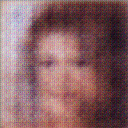
\includegraphics[width=150px]{500_fake_images/samples_5_241.png}%
\caption{A Man With A Beard Wearing A Tie}%
\end{figure}

%
\end{document}